\documentclass[twoside]{book}

% Packages required by doxygen
\usepackage{calc}
\usepackage{doxygen}
\usepackage{graphicx}
\usepackage[utf8]{inputenc}
\usepackage{makeidx}
\usepackage{multicol}
\usepackage{multirow}
\usepackage{textcomp}
\usepackage[table]{xcolor}

% Font selection
\usepackage[T1]{fontenc}
\usepackage{mathptmx}
\usepackage[scaled=.90]{helvet}
\usepackage{courier}
\usepackage{amssymb}
\usepackage{sectsty}
\renewcommand{\familydefault}{\sfdefault}
\allsectionsfont{%
  \fontseries{bc}\selectfont%
  \color{darkgray}%
}
\renewcommand{\DoxyLabelFont}{%
  \fontseries{bc}\selectfont%
  \color{darkgray}%
}

% Page & text layout
\usepackage{geometry}
\geometry{%
  a4paper,%
  top=2.5cm,%
  bottom=2.5cm,%
  left=2.5cm,%
  right=2.5cm%
}
\tolerance=750
\hfuzz=15pt
\hbadness=750
\setlength{\emergencystretch}{15pt}
\setlength{\parindent}{0cm}
\setlength{\parskip}{0.2cm}
\makeatletter
\renewcommand{\paragraph}{%
  \@startsection{paragraph}{4}{0ex}{-1.0ex}{1.0ex}{%
    \normalfont\normalsize\bfseries\SS@parafont%
  }%
}
\renewcommand{\subparagraph}{%
  \@startsection{subparagraph}{5}{0ex}{-1.0ex}{1.0ex}{%
    \normalfont\normalsize\bfseries\SS@subparafont%
  }%
}
\makeatother

% Headers & footers
\usepackage{fancyhdr}
\pagestyle{fancyplain}
\fancyhead[LE]{\fancyplain{}{\bfseries\thepage}}
\fancyhead[CE]{\fancyplain{}{}}
\fancyhead[RE]{\fancyplain{}{\bfseries\leftmark}}
\fancyhead[LO]{\fancyplain{}{\bfseries\rightmark}}
\fancyhead[CO]{\fancyplain{}{}}
\fancyhead[RO]{\fancyplain{}{\bfseries\thepage}}
\fancyfoot[LE]{\fancyplain{}{}}
\fancyfoot[CE]{\fancyplain{}{}}
\fancyfoot[RE]{\fancyplain{}{\bfseries\scriptsize Generated on Mon Mar 19 2018 22\-:59\-:09 for Topsie Texty by Doxygen }}
\fancyfoot[LO]{\fancyplain{}{\bfseries\scriptsize Generated on Mon Mar 19 2018 22\-:59\-:09 for Topsie Texty by Doxygen }}
\fancyfoot[CO]{\fancyplain{}{}}
\fancyfoot[RO]{\fancyplain{}{}}
\renewcommand{\footrulewidth}{0.4pt}
\renewcommand{\chaptermark}[1]{%
  \markboth{#1}{}%
}
\renewcommand{\sectionmark}[1]{%
  \markright{\thesection\ #1}%
}

% Indices & bibliography
\usepackage{natbib}
\usepackage[titles]{tocloft}
\setcounter{tocdepth}{3}
\setcounter{secnumdepth}{5}
\makeindex

% Hyperlinks (required, but should be loaded last)
\usepackage{ifpdf}
\ifpdf
  \usepackage[pdftex,pagebackref=true]{hyperref}
\else
  \usepackage[ps2pdf,pagebackref=true]{hyperref}
\fi
\hypersetup{%
  colorlinks=true,%
  linkcolor=blue,%
  citecolor=blue,%
  unicode%
}

% Custom commands
\newcommand{\clearemptydoublepage}{%
  \newpage{\pagestyle{empty}\cleardoublepage}%
}


%===== C O N T E N T S =====

\begin{document}

% Titlepage & ToC
\hypersetup{pageanchor=false}
\pagenumbering{roman}
\begin{titlepage}
\vspace*{7cm}
\begin{center}%
{\Large Topsie Texty }\\
\vspace*{1cm}
{\large Generated by Doxygen 1.8.5}\\
\vspace*{0.5cm}
{\small Mon Mar 19 2018 22:59:09}\\
\end{center}
\end{titlepage}
\clearemptydoublepage
\tableofcontents
\clearemptydoublepage
\pagenumbering{arabic}
\hypersetup{pageanchor=true}

%--- Begin generated contents ---
\chapter{Hierarchical Index}
\section{Class Hierarchy}
This inheritance list is sorted roughly, but not completely, alphabetically\-:\begin{DoxyCompactList}
\item \contentsline{section}{Board}{\pageref{classBoard}}{}
\begin{DoxyCompactList}
\item \contentsline{section}{Room}{\pageref{classRoom}}{}
\end{DoxyCompactList}
\item \contentsline{section}{Characters}{\pageref{classCharacters}}{}
\item \contentsline{section}{Helpers}{\pageref{classHelpers}}{}
\item \contentsline{section}{Items}{\pageref{classItems}}{}
\item \contentsline{section}{Map\-Interface}{\pageref{classMapInterface}}{}
\item \contentsline{section}{Map\-Interface1}{\pageref{classMapInterface1}}{}
\item \contentsline{section}{Puzzles}{\pageref{classPuzzles}}{}
\item \contentsline{section}{save}{\pageref{classsave}}{}
\item \contentsline{section}{Wonder\-Land}{\pageref{classWonderLand}}{}
\end{DoxyCompactList}

\chapter{Class Index}
\section{Class List}
Here are the classes, structs, unions and interfaces with brief descriptions\-:\begin{DoxyCompactList}
\item\contentsline{section}{\hyperlink{classBoard}{Board} }{\pageref{classBoard}}{}
\item\contentsline{section}{\hyperlink{classCharacters}{Characters} }{\pageref{classCharacters}}{}
\item\contentsline{section}{\hyperlink{classHelpers}{Helpers} }{\pageref{classHelpers}}{}
\item\contentsline{section}{\hyperlink{classItems}{Items} }{\pageref{classItems}}{}
\item\contentsline{section}{\hyperlink{classMapInterface}{Map\-Interface} }{\pageref{classMapInterface}}{}
\item\contentsline{section}{\hyperlink{classMapInterface1}{Map\-Interface1} }{\pageref{classMapInterface1}}{}
\item\contentsline{section}{\hyperlink{classPuzzles}{Puzzles} }{\pageref{classPuzzles}}{}
\item\contentsline{section}{\hyperlink{classRoom}{Room} }{\pageref{classRoom}}{}
\item\contentsline{section}{\hyperlink{classsave}{save} }{\pageref{classsave}}{}
\item\contentsline{section}{\hyperlink{classWonderLand}{Wonder\-Land} }{\pageref{classWonderLand}}{}
\end{DoxyCompactList}

\chapter{File Index}
\section{File List}
Here is a list of all files with brief descriptions\-:\begin{DoxyCompactList}
\item\contentsline{section}{include/\hyperlink{Board_8h}{Board.\-h} }{\pageref{Board_8h}}{}
\item\contentsline{section}{include/\hyperlink{Characters_8h}{Characters.\-h} }{\pageref{Characters_8h}}{}
\item\contentsline{section}{include/\hyperlink{Helpers_8h}{Helpers.\-h} }{\pageref{Helpers_8h}}{}
\item\contentsline{section}{include/\hyperlink{Items_8h}{Items.\-h} }{\pageref{Items_8h}}{}
\item\contentsline{section}{include/\hyperlink{MapInterface_8h}{Map\-Interface.\-h} }{\pageref{MapInterface_8h}}{}
\item\contentsline{section}{include/\hyperlink{puzzles_8h}{puzzles.\-h} }{\pageref{puzzles_8h}}{}
\item\contentsline{section}{include/\hyperlink{Room_8h}{Room.\-h} }{\pageref{Room_8h}}{}
\item\contentsline{section}{include/\hyperlink{SaveFunction_8h}{Save\-Function.\-h} }{\pageref{SaveFunction_8h}}{}
\item\contentsline{section}{include/\hyperlink{WonderLand_8h}{Wonder\-Land.\-h} }{\pageref{WonderLand_8h}}{}
\item\contentsline{section}{src/\hyperlink{Characters_8cpp}{Characters.\-cpp} }{\pageref{Characters_8cpp}}{}
\item\contentsline{section}{src/\hyperlink{Helpers_8cpp}{Helpers.\-cpp} }{\pageref{Helpers_8cpp}}{}
\item\contentsline{section}{src/\hyperlink{Items_8cpp}{Items.\-cpp} }{\pageref{Items_8cpp}}{}
\item\contentsline{section}{src/\hyperlink{MapInterface-IMP_8cpp}{Map\-Interface-\/\-I\-M\-P.\-cpp} }{\pageref{MapInterface-IMP_8cpp}}{}
\item\contentsline{section}{src/\hyperlink{puzzles_8cpp}{puzzles.\-cpp} }{\pageref{puzzles_8cpp}}{}
\item\contentsline{section}{src/\hyperlink{Room-IMP_8cpp}{Room-\/\-I\-M\-P.\-cpp} }{\pageref{Room-IMP_8cpp}}{}
\item\contentsline{section}{src/\hyperlink{SaveFunction_8cpp}{Save\-Function.\-cpp} }{\pageref{SaveFunction_8cpp}}{}
\item\contentsline{section}{src/\hyperlink{WonderLand-IMP_8cpp}{Wonder\-Land-\/\-I\-M\-P.\-cpp} }{\pageref{WonderLand-IMP_8cpp}}{}
\item\contentsline{section}{src/\hyperlink{WonderMain_8cpp}{Wonder\-Main.\-cpp} }{\pageref{WonderMain_8cpp}}{}
\end{DoxyCompactList}

\chapter{Class Documentation}
\hypertarget{classBoard}{\section{Board Class Reference}
\label{classBoard}\index{Board@{Board}}
}


{\ttfamily \#include $<$Board.\-h$>$}

Inheritance diagram for Board\-:\begin{figure}[H]
\begin{center}
\leavevmode
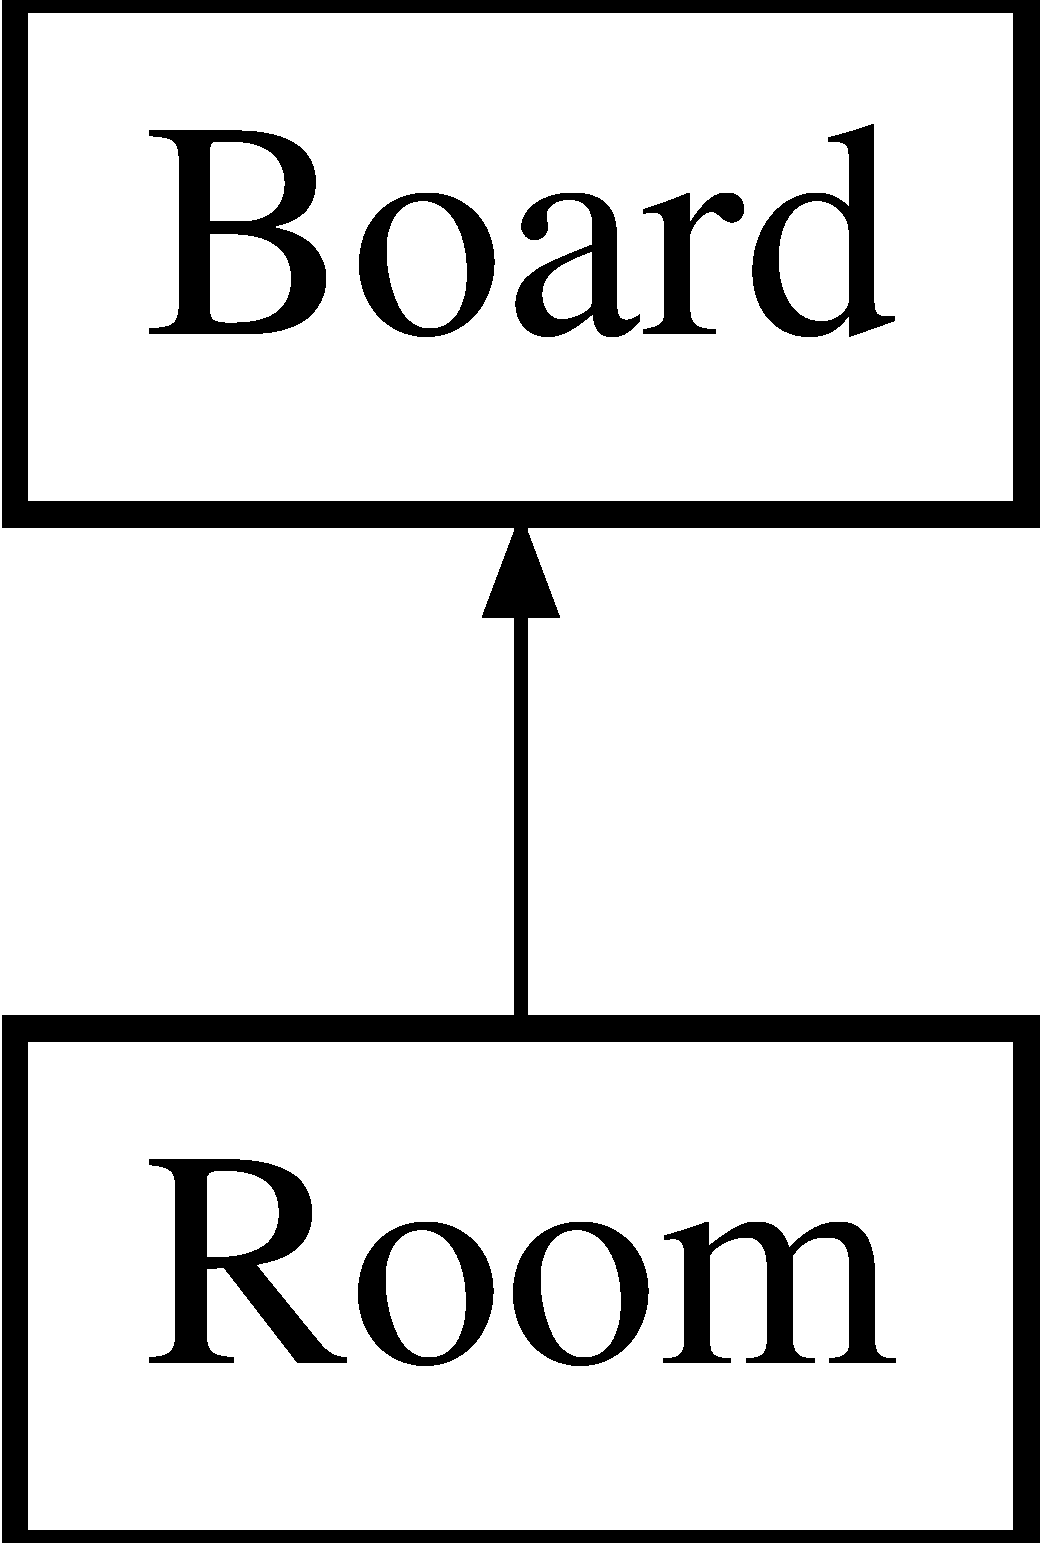
\includegraphics[height=2.000000cm]{classBoard}
\end{center}
\end{figure}
\subsection*{Public Attributes}
\begin{DoxyCompactItemize}
\item 
int \hyperlink{classBoard_a0a98d341c4c8f9e5ef513364f4453112}{Layout} \mbox{[}$\,$\mbox{]}\mbox{[}5\mbox{]}
\end{DoxyCompactItemize}


\subsection{Member Data Documentation}
\hypertarget{classBoard_a0a98d341c4c8f9e5ef513364f4453112}{\index{Board@{Board}!Layout@{Layout}}
\index{Layout@{Layout}!Board@{Board}}
\subsubsection[{Layout}]{\setlength{\rightskip}{0pt plus 5cm}int Board\-::\-Layout\mbox{[}$\,$\mbox{]}\mbox{[}5\mbox{]}}}\label{classBoard_a0a98d341c4c8f9e5ef513364f4453112}


The documentation for this class was generated from the following file\-:\begin{DoxyCompactItemize}
\item 
include/\hyperlink{Board_8h}{Board.\-h}\end{DoxyCompactItemize}

\hypertarget{classCharacters}{\section{Characters Class Reference}
\label{classCharacters}\index{Characters@{Characters}}
}


{\ttfamily \#include $<$Characters.\-h$>$}

\subsection*{Public Member Functions}
\begin{DoxyCompactItemize}
\item 
\hyperlink{classCharacters_a982bd095e88521e33817bc3ac4eb9607}{Characters} (int)
\item 
\hyperlink{classCharacters_a265d04d1ad3a6f8d0ca8fd619cfa507a}{Characters} (string)
\item 
bool \hyperlink{classCharacters_a9ba4cc578a1a39b99aa768687a4f61d3}{interact} ()
\item 
bool \hyperlink{classCharacters_a4ebc19878bbf951f7c5f2bcebca7a7f8}{travel} (\hyperlink{classMapInterface}{Map\-Interface} \&)
\item 
bool \hyperlink{classCharacters_af427bea62ac1676a045b99e91a2955ee}{fight} (\hyperlink{classCharacters}{Characters})
\item 
string \hyperlink{classCharacters_ade67cb33a8d5a9f71cf5d74d36c9334c}{get\-Name} ()
\item 
double \hyperlink{classCharacters_a01416ed6aa653ac13d321debe0d87710}{get\-Location} ()
\item 
int \hyperlink{classCharacters_a4fcf7eddcf088020e4f6fec769c2f656}{get\-Health} ()
\item 
int \hyperlink{classCharacters_a6903ebf441ed1de576019be728915a39}{get\-Strength} ()
\item 
void \hyperlink{classCharacters_afcdf7a6bd55be44e1da4e8b82418c162}{lose\-Health} (int)
\item 
void \hyperlink{classCharacters_ab5e230273f1224917c45d64bd475b2b3}{gain\-Health} (int)
\item 
void \hyperlink{classCharacters_a78c7c420c9fb868cc8b43874d3d89abd}{gain\-Strength} (int)
\end{DoxyCompactItemize}


\subsection{Constructor \& Destructor Documentation}
\hypertarget{classCharacters_a982bd095e88521e33817bc3ac4eb9607}{\index{Characters@{Characters}!Characters@{Characters}}
\index{Characters@{Characters}!Characters@{Characters}}
\subsubsection[{Characters}]{\setlength{\rightskip}{0pt plus 5cm}Characters\-::\-Characters (
\begin{DoxyParamCaption}
\item[{int}]{choice}
\end{DoxyParamCaption}
)}}\label{classCharacters_a982bd095e88521e33817bc3ac4eb9607}
\begin{DoxyPrecond}{Precondition}
none 
\end{DoxyPrecond}
\begin{DoxyPostcond}{Postcondition}
creates Character object 
\end{DoxyPostcond}

\begin{DoxyParams}{Parameters}
{\em int} & to signify which Character \\
\hline
\end{DoxyParams}
\hypertarget{classCharacters_a265d04d1ad3a6f8d0ca8fd619cfa507a}{\index{Characters@{Characters}!Characters@{Characters}}
\index{Characters@{Characters}!Characters@{Characters}}
\subsubsection[{Characters}]{\setlength{\rightskip}{0pt plus 5cm}Characters\-::\-Characters (
\begin{DoxyParamCaption}
\item[{string}]{set\-Name}
\end{DoxyParamCaption}
)}}\label{classCharacters_a265d04d1ad3a6f8d0ca8fd619cfa507a}
\begin{DoxyPrecond}{Precondition}
none 
\end{DoxyPrecond}
\begin{DoxyPostcond}{Postcondition}
creates enemy character object 
\end{DoxyPostcond}

\begin{DoxyParams}{Parameters}
{\em string} & for enemy name and pointer to \hyperlink{classMapInterface}{Map\-Interface} for their location \\
\hline
\end{DoxyParams}


\subsection{Member Function Documentation}
\hypertarget{classCharacters_af427bea62ac1676a045b99e91a2955ee}{\index{Characters@{Characters}!fight@{fight}}
\index{fight@{fight}!Characters@{Characters}}
\subsubsection[{fight}]{\setlength{\rightskip}{0pt plus 5cm}bool Characters\-::fight (
\begin{DoxyParamCaption}
\item[{{\bf Characters}}]{enemy}
\end{DoxyParamCaption}
)}}\label{classCharacters_af427bea62ac1676a045b99e91a2955ee}
\begin{DoxyPrecond}{Precondition}
both characters must be initiated 
\end{DoxyPrecond}
\begin{DoxyPostcond}{Postcondition}
reduces both healths until one reaches zero and the other wins 
\end{DoxyPostcond}

\begin{DoxyParams}{Parameters}
{\em enemy} & character object \\
\hline
\end{DoxyParams}
\begin{DoxyReturn}{Returns}
bool to signify successful fight 
\end{DoxyReturn}
\hypertarget{classCharacters_ab5e230273f1224917c45d64bd475b2b3}{\index{Characters@{Characters}!gain\-Health@{gain\-Health}}
\index{gain\-Health@{gain\-Health}!Characters@{Characters}}
\subsubsection[{gain\-Health}]{\setlength{\rightskip}{0pt plus 5cm}void Characters\-::gain\-Health (
\begin{DoxyParamCaption}
\item[{int}]{gain}
\end{DoxyParamCaption}
)}}\label{classCharacters_ab5e230273f1224917c45d64bd475b2b3}
\begin{DoxyPrecond}{Precondition}
character is initiated and health is set 
\end{DoxyPrecond}
\begin{DoxyPostcond}{Postcondition}
health is increased by parameter 
\end{DoxyPostcond}
\hypertarget{classCharacters_a78c7c420c9fb868cc8b43874d3d89abd}{\index{Characters@{Characters}!gain\-Strength@{gain\-Strength}}
\index{gain\-Strength@{gain\-Strength}!Characters@{Characters}}
\subsubsection[{gain\-Strength}]{\setlength{\rightskip}{0pt plus 5cm}void Characters\-::gain\-Strength (
\begin{DoxyParamCaption}
\item[{int}]{gain}
\end{DoxyParamCaption}
)}}\label{classCharacters_a78c7c420c9fb868cc8b43874d3d89abd}
\begin{DoxyPrecond}{Precondition}
character is initiated and strength is set 
\end{DoxyPrecond}
\begin{DoxyPostcond}{Postcondition}
strength is increased by parameter 
\end{DoxyPostcond}
\hypertarget{classCharacters_a4fcf7eddcf088020e4f6fec769c2f656}{\index{Characters@{Characters}!get\-Health@{get\-Health}}
\index{get\-Health@{get\-Health}!Characters@{Characters}}
\subsubsection[{get\-Health}]{\setlength{\rightskip}{0pt plus 5cm}int Characters\-::get\-Health (
\begin{DoxyParamCaption}
{}
\end{DoxyParamCaption}
)}}\label{classCharacters_a4fcf7eddcf088020e4f6fec769c2f656}
\begin{DoxyPrecond}{Precondition}
character is initiated and health is set 
\end{DoxyPrecond}
\begin{DoxyPostcond}{Postcondition}
gets health value 
\end{DoxyPostcond}
\begin{DoxyReturn}{Returns}
int 
\end{DoxyReturn}
\hypertarget{classCharacters_a01416ed6aa653ac13d321debe0d87710}{\index{Characters@{Characters}!get\-Location@{get\-Location}}
\index{get\-Location@{get\-Location}!Characters@{Characters}}
\subsubsection[{get\-Location}]{\setlength{\rightskip}{0pt plus 5cm}double Characters\-::get\-Location (
\begin{DoxyParamCaption}
{}
\end{DoxyParamCaption}
)}}\label{classCharacters_a01416ed6aa653ac13d321debe0d87710}
\begin{DoxyPrecond}{Precondition}
character is initiated and location is set 
\end{DoxyPrecond}
\begin{DoxyPostcond}{Postcondition}
gets location value 
\end{DoxyPostcond}
\begin{DoxyReturn}{Returns}
double 
\end{DoxyReturn}
\hypertarget{classCharacters_ade67cb33a8d5a9f71cf5d74d36c9334c}{\index{Characters@{Characters}!get\-Name@{get\-Name}}
\index{get\-Name@{get\-Name}!Characters@{Characters}}
\subsubsection[{get\-Name}]{\setlength{\rightskip}{0pt plus 5cm}string Characters\-::get\-Name (
\begin{DoxyParamCaption}
{}
\end{DoxyParamCaption}
)}}\label{classCharacters_ade67cb33a8d5a9f71cf5d74d36c9334c}
\begin{DoxyPrecond}{Precondition}
character is initiated and name is set 
\end{DoxyPrecond}
\begin{DoxyPostcond}{Postcondition}
gets name 
\end{DoxyPostcond}
\begin{DoxyReturn}{Returns}
string 
\end{DoxyReturn}
\hypertarget{classCharacters_a6903ebf441ed1de576019be728915a39}{\index{Characters@{Characters}!get\-Strength@{get\-Strength}}
\index{get\-Strength@{get\-Strength}!Characters@{Characters}}
\subsubsection[{get\-Strength}]{\setlength{\rightskip}{0pt plus 5cm}int Characters\-::get\-Strength (
\begin{DoxyParamCaption}
{}
\end{DoxyParamCaption}
)}}\label{classCharacters_a6903ebf441ed1de576019be728915a39}
\begin{DoxyPrecond}{Precondition}
character is initiated and strength is set 
\end{DoxyPrecond}
\begin{DoxyPostcond}{Postcondition}
gets strength value 
\end{DoxyPostcond}
\begin{DoxyReturn}{Returns}
int 
\end{DoxyReturn}
\hypertarget{classCharacters_a9ba4cc578a1a39b99aa768687a4f61d3}{\index{Characters@{Characters}!interact@{interact}}
\index{interact@{interact}!Characters@{Characters}}
\subsubsection[{interact}]{\setlength{\rightskip}{0pt plus 5cm}bool Characters\-::interact (
\begin{DoxyParamCaption}
{}
\end{DoxyParamCaption}
)}}\label{classCharacters_a9ba4cc578a1a39b99aa768687a4f61d3}
\hypertarget{classCharacters_afcdf7a6bd55be44e1da4e8b82418c162}{\index{Characters@{Characters}!lose\-Health@{lose\-Health}}
\index{lose\-Health@{lose\-Health}!Characters@{Characters}}
\subsubsection[{lose\-Health}]{\setlength{\rightskip}{0pt plus 5cm}void Characters\-::lose\-Health (
\begin{DoxyParamCaption}
\item[{int}]{loss}
\end{DoxyParamCaption}
)}}\label{classCharacters_afcdf7a6bd55be44e1da4e8b82418c162}
\begin{DoxyPrecond}{Precondition}
character is initiated and health is set 
\end{DoxyPrecond}
\begin{DoxyPostcond}{Postcondition}
health is diminished by parameter 
\end{DoxyPostcond}
\hypertarget{classCharacters_a4ebc19878bbf951f7c5f2bcebca7a7f8}{\index{Characters@{Characters}!travel@{travel}}
\index{travel@{travel}!Characters@{Characters}}
\subsubsection[{travel}]{\setlength{\rightskip}{0pt plus 5cm}bool Characters\-::travel (
\begin{DoxyParamCaption}
\item[{{\bf Map\-Interface} \&}]{}
\end{DoxyParamCaption}
)}}\label{classCharacters_a4ebc19878bbf951f7c5f2bcebca7a7f8}
\begin{DoxyPrecond}{Precondition}
character is initiated and parameter is of type \hyperlink{classMapInterface}{Map\-Interface} 
\end{DoxyPrecond}
\begin{DoxyPostcond}{Postcondition}
changes location of Character 
\end{DoxyPostcond}

\begin{DoxyParams}{Parameters}
{\em \hyperlink{classMapInterface}{Map\-Interface}} & \\
\hline
\end{DoxyParams}
\begin{DoxyReturn}{Returns}
bool 
\end{DoxyReturn}


The documentation for this class was generated from the following files\-:\begin{DoxyCompactItemize}
\item 
include/\hyperlink{Characters_8h}{Characters.\-h}\item 
src/\hyperlink{Characters_8cpp}{Characters.\-cpp}\end{DoxyCompactItemize}

\hypertarget{classHelpers}{\section{Helpers Class Reference}
\label{classHelpers}\index{Helpers@{Helpers}}
}


{\ttfamily \#include $<$Helpers.\-h$>$}

\subsection*{Public Member Functions}
\begin{DoxyCompactItemize}
\item 
\hyperlink{classHelpers_aa1ef3c3323aa6c76cf060bdff03920ad}{Helpers} (string)
\item 
int \hyperlink{classHelpers_a93876ddf85e62d0520fe82b48137579e}{speak} ()
\end{DoxyCompactItemize}


\subsection{Constructor \& Destructor Documentation}
\hypertarget{classHelpers_aa1ef3c3323aa6c76cf060bdff03920ad}{\index{Helpers@{Helpers}!Helpers@{Helpers}}
\index{Helpers@{Helpers}!Helpers@{Helpers}}
\subsubsection[{Helpers}]{\setlength{\rightskip}{0pt plus 5cm}Helpers\-::\-Helpers (
\begin{DoxyParamCaption}
\item[{string}]{charact}
\end{DoxyParamCaption}
)}}\label{classHelpers_aa1ef3c3323aa6c76cf060bdff03920ad}
\begin{DoxyPrecond}{Precondition}
none 
\end{DoxyPrecond}
\begin{DoxyPostcond}{Postcondition}
creates helper character 
\end{DoxyPostcond}

\begin{DoxyParams}{Parameters}
{\em string} & for name \\
\hline
\end{DoxyParams}


\subsection{Member Function Documentation}
\hypertarget{classHelpers_a93876ddf85e62d0520fe82b48137579e}{\index{Helpers@{Helpers}!speak@{speak}}
\index{speak@{speak}!Helpers@{Helpers}}
\subsubsection[{speak}]{\setlength{\rightskip}{0pt plus 5cm}int Helpers\-::speak (
\begin{DoxyParamCaption}
{}
\end{DoxyParamCaption}
)}}\label{classHelpers_a93876ddf85e62d0520fe82b48137579e}
\begin{DoxyPrecond}{Precondition}
helper is initiated 
\end{DoxyPrecond}
\begin{DoxyPostcond}{Postcondition}
outputs dialogue of helper 
\end{DoxyPostcond}
\begin{DoxyReturn}{Returns}
int for next command 
\end{DoxyReturn}


The documentation for this class was generated from the following files\-:\begin{DoxyCompactItemize}
\item 
include/\hyperlink{Helpers_8h}{Helpers.\-h}\item 
src/\hyperlink{Helpers_8cpp}{Helpers.\-cpp}\end{DoxyCompactItemize}

\hypertarget{classItems}{\section{Items Class Reference}
\label{classItems}\index{Items@{Items}}
}


{\ttfamily \#include $<$Items.\-h$>$}

\subsection*{Public Member Functions}
\begin{DoxyCompactItemize}
\item 
\hyperlink{classItems_a3d368c3c7a14eb2a038682bd4da5d41a}{Items} ()
\item 
int \hyperlink{classItems_af8655af10bb8469490cbc917d4f00c8a}{Enlarging\-Food} (\hyperlink{classCharacters}{Characters})
\item 
int \hyperlink{classItems_ac14b387a29dee52097bef458b7ef4e82}{Shrinking\-Food} (\hyperlink{classCharacters}{Characters})
\item 
int \hyperlink{classItems_a1038dc083b26bcfd5bdd148e72a68bcc}{Hatter\-Hat} (\hyperlink{classCharacters}{Characters})
\item 
int \hyperlink{classItems_ac6ddd28ed44d321de086b63d21e33771}{Key} (\hyperlink{classCharacters}{Characters})
\item 
int \hyperlink{classItems_a2951a091c7c7b3f04b0c11b0e15b6b0a}{Hatter\-Sword} (\hyperlink{classCharacters}{Characters})
\end{DoxyCompactItemize}


\subsection{Constructor \& Destructor Documentation}
\hypertarget{classItems_a3d368c3c7a14eb2a038682bd4da5d41a}{\index{Items@{Items}!Items@{Items}}
\index{Items@{Items}!Items@{Items}}
\subsubsection[{Items}]{\setlength{\rightskip}{0pt plus 5cm}Items\-::\-Items (
\begin{DoxyParamCaption}
{}
\end{DoxyParamCaption}
)}}\label{classItems_a3d368c3c7a14eb2a038682bd4da5d41a}
\begin{DoxyPrecond}{Precondition}
none 
\end{DoxyPrecond}
\begin{DoxyPostcond}{Postcondition}
creates \hyperlink{classItems}{Items} object(\-Default) 
\end{DoxyPostcond}


\subsection{Member Function Documentation}
\hypertarget{classItems_af8655af10bb8469490cbc917d4f00c8a}{\index{Items@{Items}!Enlarging\-Food@{Enlarging\-Food}}
\index{Enlarging\-Food@{Enlarging\-Food}!Items@{Items}}
\subsubsection[{Enlarging\-Food}]{\setlength{\rightskip}{0pt plus 5cm}int Items\-::\-Enlarging\-Food (
\begin{DoxyParamCaption}
\item[{{\bf Characters}}]{a}
\end{DoxyParamCaption}
)}}\label{classItems_af8655af10bb8469490cbc917d4f00c8a}
\begin{DoxyPrecond}{Precondition}
Can be Found on a Map 
\end{DoxyPrecond}
\begin{DoxyPostcond}{Postcondition}
Increases Your H\-E\-A\-L\-T\-H 
\end{DoxyPostcond}

\begin{DoxyParams}{Parameters}
{\em Character} & Class \\
\hline
\end{DoxyParams}
\hypertarget{classItems_a1038dc083b26bcfd5bdd148e72a68bcc}{\index{Items@{Items}!Hatter\-Hat@{Hatter\-Hat}}
\index{Hatter\-Hat@{Hatter\-Hat}!Items@{Items}}
\subsubsection[{Hatter\-Hat}]{\setlength{\rightskip}{0pt plus 5cm}int Items\-::\-Hatter\-Hat (
\begin{DoxyParamCaption}
\item[{{\bf Characters}}]{h}
\end{DoxyParamCaption}
)}}\label{classItems_a1038dc083b26bcfd5bdd148e72a68bcc}
\begin{DoxyPrecond}{Precondition}
Can be Found on a Map 
\end{DoxyPrecond}
\begin{DoxyPostcond}{Postcondition}
Increases Your S\-T\-R\-E\-N\-G\-T\-H 
\end{DoxyPostcond}

\begin{DoxyParams}{Parameters}
{\em Character} & Class \\
\hline
\end{DoxyParams}
\hypertarget{classItems_a2951a091c7c7b3f04b0c11b0e15b6b0a}{\index{Items@{Items}!Hatter\-Sword@{Hatter\-Sword}}
\index{Hatter\-Sword@{Hatter\-Sword}!Items@{Items}}
\subsubsection[{Hatter\-Sword}]{\setlength{\rightskip}{0pt plus 5cm}int Items\-::\-Hatter\-Sword (
\begin{DoxyParamCaption}
\item[{{\bf Characters}}]{s}
\end{DoxyParamCaption}
)}}\label{classItems_a2951a091c7c7b3f04b0c11b0e15b6b0a}
\begin{DoxyPrecond}{Precondition}
Can be Found on a Map 
\end{DoxyPrecond}
\begin{DoxyPostcond}{Postcondition}
Increases Your Strength and Health 
\end{DoxyPostcond}

\begin{DoxyParams}{Parameters}
{\em Character} & Class \\
\hline
\end{DoxyParams}
\hypertarget{classItems_ac6ddd28ed44d321de086b63d21e33771}{\index{Items@{Items}!Key@{Key}}
\index{Key@{Key}!Items@{Items}}
\subsubsection[{Key}]{\setlength{\rightskip}{0pt plus 5cm}int Items\-::\-Key (
\begin{DoxyParamCaption}
\item[{{\bf Characters}}]{k}
\end{DoxyParamCaption}
)}}\label{classItems_ac6ddd28ed44d321de086b63d21e33771}
\begin{DoxyPrecond}{Precondition}
Can be Found on a Map 
\end{DoxyPrecond}
\begin{DoxyPostcond}{Postcondition}
Increases Your S\-T\-R\-E\-N\-G\-T\-H 
\end{DoxyPostcond}

\begin{DoxyParams}{Parameters}
{\em Character} & Class \\
\hline
\end{DoxyParams}
\hypertarget{classItems_ac14b387a29dee52097bef458b7ef4e82}{\index{Items@{Items}!Shrinking\-Food@{Shrinking\-Food}}
\index{Shrinking\-Food@{Shrinking\-Food}!Items@{Items}}
\subsubsection[{Shrinking\-Food}]{\setlength{\rightskip}{0pt plus 5cm}int Items\-::\-Shrinking\-Food (
\begin{DoxyParamCaption}
\item[{{\bf Characters}}]{s}
\end{DoxyParamCaption}
)}}\label{classItems_ac14b387a29dee52097bef458b7ef4e82}
\begin{DoxyPrecond}{Precondition}
Can be Found on a Map 
\end{DoxyPrecond}
\begin{DoxyPostcond}{Postcondition}
Decreases Your H\-E\-A\-L\-T\-H 
\end{DoxyPostcond}

\begin{DoxyParams}{Parameters}
{\em Character} & Class \\
\hline
\end{DoxyParams}


The documentation for this class was generated from the following files\-:\begin{DoxyCompactItemize}
\item 
include/\hyperlink{Items_8h}{Items.\-h}\item 
src/\hyperlink{Items_8cpp}{Items.\-cpp}\end{DoxyCompactItemize}

\hypertarget{classMapInterface}{\section{Map\-Interface Class Reference}
\label{classMapInterface}\index{Map\-Interface@{Map\-Interface}}
}


{\ttfamily \#include $<$Map\-Interface.\-h$>$}

\subsection*{Public Member Functions}
\begin{DoxyCompactItemize}
\item 
void \hyperlink{classMapInterface_a6767872fad1ca9b0fcf1944408a8f467}{move} (int i, \hyperlink{classWonderLand}{Wonder\-Land} \&p)
\item 
void \hyperlink{classMapInterface_a984271455cbaa25a6ce75935a60f0784}{return\-Info} (\hyperlink{classWonderLand}{Wonder\-Land} \&p, \hyperlink{classRoom}{Room} \&b)
\end{DoxyCompactItemize}


\subsection{Member Function Documentation}
\hypertarget{classMapInterface_a6767872fad1ca9b0fcf1944408a8f467}{\index{Map\-Interface@{Map\-Interface}!move@{move}}
\index{move@{move}!MapInterface@{Map\-Interface}}
\subsubsection[{move}]{\setlength{\rightskip}{0pt plus 5cm}void Map\-Interface\-::move (
\begin{DoxyParamCaption}
\item[{int}]{i, }
\item[{{\bf Wonder\-Land} \&}]{p}
\end{DoxyParamCaption}
)}}\label{classMapInterface_a6767872fad1ca9b0fcf1944408a8f467}
\begin{DoxyPrecond}{Precondition}
wonderland exists 
\end{DoxyPrecond}
\begin{DoxyPostcond}{Postcondition}
moves your location within the room 
\end{DoxyPostcond}

\begin{DoxyParams}{Parameters}
{\em int} & is direction to move, p represents the map \\
\hline
\end{DoxyParams}
\hypertarget{classMapInterface_a984271455cbaa25a6ce75935a60f0784}{\index{Map\-Interface@{Map\-Interface}!return\-Info@{return\-Info}}
\index{return\-Info@{return\-Info}!MapInterface@{Map\-Interface}}
\subsubsection[{return\-Info}]{\setlength{\rightskip}{0pt plus 5cm}void Map\-Interface\-::return\-Info (
\begin{DoxyParamCaption}
\item[{{\bf Wonder\-Land} \&}]{p, }
\item[{{\bf Room} \&}]{b}
\end{DoxyParamCaption}
)}}\label{classMapInterface_a984271455cbaa25a6ce75935a60f0784}
\begin{DoxyPrecond}{Precondition}
wonderland exists 
\end{DoxyPrecond}
\begin{DoxyPostcond}{Postcondition}
returns which room and coordinates of your location 
\end{DoxyPostcond}

\begin{DoxyParams}{Parameters}
{\em p} & represents the map, b is the room you're in \\
\hline
\end{DoxyParams}


The documentation for this class was generated from the following files\-:\begin{DoxyCompactItemize}
\item 
include/\hyperlink{MapInterface_8h}{Map\-Interface.\-h}\item 
src/\hyperlink{MapInterface-IMP_8cpp}{Map\-Interface-\/\-I\-M\-P.\-cpp}\end{DoxyCompactItemize}

\hypertarget{classMapInterface1}{\section{Map\-Interface1 Class Reference}
\label{classMapInterface1}\index{Map\-Interface1@{Map\-Interface1}}
}


{\ttfamily \#include $<$Characters.\-h$>$}

\subsection*{Public Member Functions}
\begin{DoxyCompactItemize}
\item 
\hyperlink{classMapInterface1_a925e7c7524ae7bf43a9dc05e2ce05e62}{Map\-Interface1} ()
\item 
double \hyperlink{classMapInterface1_a6069e9ce09b291c1b41ba9ad6c63c980}{get\-Info} ()
\end{DoxyCompactItemize}


\subsection{Constructor \& Destructor Documentation}
\hypertarget{classMapInterface1_a925e7c7524ae7bf43a9dc05e2ce05e62}{\index{Map\-Interface1@{Map\-Interface1}!Map\-Interface1@{Map\-Interface1}}
\index{Map\-Interface1@{Map\-Interface1}!MapInterface1@{Map\-Interface1}}
\subsubsection[{Map\-Interface1}]{\setlength{\rightskip}{0pt plus 5cm}Map\-Interface1\-::\-Map\-Interface1 (
\begin{DoxyParamCaption}
{}
\end{DoxyParamCaption}
)\hspace{0.3cm}{\ttfamily [inline]}}}\label{classMapInterface1_a925e7c7524ae7bf43a9dc05e2ce05e62}


\subsection{Member Function Documentation}
\hypertarget{classMapInterface1_a6069e9ce09b291c1b41ba9ad6c63c980}{\index{Map\-Interface1@{Map\-Interface1}!get\-Info@{get\-Info}}
\index{get\-Info@{get\-Info}!MapInterface1@{Map\-Interface1}}
\subsubsection[{get\-Info}]{\setlength{\rightskip}{0pt plus 5cm}double Map\-Interface1\-::get\-Info (
\begin{DoxyParamCaption}
{}
\end{DoxyParamCaption}
)\hspace{0.3cm}{\ttfamily [inline]}}}\label{classMapInterface1_a6069e9ce09b291c1b41ba9ad6c63c980}


The documentation for this class was generated from the following file\-:\begin{DoxyCompactItemize}
\item 
include/\hyperlink{Characters_8h}{Characters.\-h}\end{DoxyCompactItemize}

\hypertarget{classPuzzles}{\section{Puzzles Class Reference}
\label{classPuzzles}\index{Puzzles@{Puzzles}}
}


{\ttfamily \#include $<$puzzles.\-h$>$}

\subsection*{Public Member Functions}
\begin{DoxyCompactItemize}
\item 
\hyperlink{classPuzzles_a8eeb0a6887d93a463ca5745322fe3511}{Puzzles} ()
\item 
int \hyperlink{classPuzzles_aadeec158f07b4a95efc7e70a749a9a0f}{Puzzle1} ()
\item 
int \hyperlink{classPuzzles_ad5abbf71069a85987b2de04f8fdfa108}{Puzzle2} ()
\item 
int \hyperlink{classPuzzles_ac7df2bc196125c11ece278f44d240538}{Puzzle3} ()
\item 
int \hyperlink{classPuzzles_a86ab262bdfed721a7932435b9329b9d6}{Puzzle4} ()
\item 
int \hyperlink{classPuzzles_aa6847c5f979faf839b4ac646e8cd5f53}{Puzzle5} ()
\item 
int \hyperlink{classPuzzles_a3bf9f67def2d876db4c77824bba588dc}{Puzzle6} ()
\item 
int \hyperlink{classPuzzles_ac6ba9d339b102ee33d110b79417c7d2f}{Puzzle7} ()
\item 
int \hyperlink{classPuzzles_a81d8a9b01494daa9397581dac6427b10}{Puzzle8} ()
\end{DoxyCompactItemize}


\subsection{Constructor \& Destructor Documentation}
\hypertarget{classPuzzles_a8eeb0a6887d93a463ca5745322fe3511}{\index{Puzzles@{Puzzles}!Puzzles@{Puzzles}}
\index{Puzzles@{Puzzles}!Puzzles@{Puzzles}}
\subsubsection[{Puzzles}]{\setlength{\rightskip}{0pt plus 5cm}Puzzles\-::\-Puzzles (
\begin{DoxyParamCaption}
{}
\end{DoxyParamCaption}
)}}\label{classPuzzles_a8eeb0a6887d93a463ca5745322fe3511}
\begin{DoxyPrecond}{Precondition}
none 
\end{DoxyPrecond}
\begin{DoxyPostcond}{Postcondition}
creates Puzzle objects 
\end{DoxyPostcond}

\begin{DoxyParams}{Parameters}
{\em none} & \\
\hline
\end{DoxyParams}


\subsection{Member Function Documentation}
\hypertarget{classPuzzles_aadeec158f07b4a95efc7e70a749a9a0f}{\index{Puzzles@{Puzzles}!Puzzle1@{Puzzle1}}
\index{Puzzle1@{Puzzle1}!Puzzles@{Puzzles}}
\subsubsection[{Puzzle1}]{\setlength{\rightskip}{0pt plus 5cm}int Puzzles\-::\-Puzzle1 (
\begin{DoxyParamCaption}
{}
\end{DoxyParamCaption}
)}}\label{classPuzzles_aadeec158f07b4a95efc7e70a749a9a0f}
\begin{DoxyPrecond}{Precondition}
none 
\end{DoxyPrecond}
\begin{DoxyPostcond}{Postcondition}
1st Puzzle(\-About Series) 
\end{DoxyPostcond}

\begin{DoxyParams}{Parameters}
{\em none} & \\
\hline
\end{DoxyParams}
\hypertarget{classPuzzles_ad5abbf71069a85987b2de04f8fdfa108}{\index{Puzzles@{Puzzles}!Puzzle2@{Puzzle2}}
\index{Puzzle2@{Puzzle2}!Puzzles@{Puzzles}}
\subsubsection[{Puzzle2}]{\setlength{\rightskip}{0pt plus 5cm}int Puzzles\-::\-Puzzle2 (
\begin{DoxyParamCaption}
{}
\end{DoxyParamCaption}
)}}\label{classPuzzles_ad5abbf71069a85987b2de04f8fdfa108}
\begin{DoxyPrecond}{Precondition}
none 
\end{DoxyPrecond}
\begin{DoxyPostcond}{Postcondition}
2nd Puzzle(\-Shapes) 
\end{DoxyPostcond}

\begin{DoxyParams}{Parameters}
{\em none} & \\
\hline
\end{DoxyParams}
\hypertarget{classPuzzles_ac7df2bc196125c11ece278f44d240538}{\index{Puzzles@{Puzzles}!Puzzle3@{Puzzle3}}
\index{Puzzle3@{Puzzle3}!Puzzles@{Puzzles}}
\subsubsection[{Puzzle3}]{\setlength{\rightskip}{0pt plus 5cm}int Puzzles\-::\-Puzzle3 (
\begin{DoxyParamCaption}
{}
\end{DoxyParamCaption}
)}}\label{classPuzzles_ac7df2bc196125c11ece278f44d240538}
\begin{DoxyPrecond}{Precondition}
none 
\end{DoxyPrecond}
\begin{DoxyPostcond}{Postcondition}
3rd Puzzle(\-Pot) 
\end{DoxyPostcond}

\begin{DoxyParams}{Parameters}
{\em none} & \\
\hline
\end{DoxyParams}
\hypertarget{classPuzzles_a86ab262bdfed721a7932435b9329b9d6}{\index{Puzzles@{Puzzles}!Puzzle4@{Puzzle4}}
\index{Puzzle4@{Puzzle4}!Puzzles@{Puzzles}}
\subsubsection[{Puzzle4}]{\setlength{\rightskip}{0pt plus 5cm}int Puzzles\-::\-Puzzle4 (
\begin{DoxyParamCaption}
{}
\end{DoxyParamCaption}
)}}\label{classPuzzles_a86ab262bdfed721a7932435b9329b9d6}
\begin{DoxyPrecond}{Precondition}
none 
\end{DoxyPrecond}
\begin{DoxyPostcond}{Postcondition}
4th Puzzle(\-Probability) 
\end{DoxyPostcond}

\begin{DoxyParams}{Parameters}
{\em none} & \\
\hline
\end{DoxyParams}
\hypertarget{classPuzzles_aa6847c5f979faf839b4ac646e8cd5f53}{\index{Puzzles@{Puzzles}!Puzzle5@{Puzzle5}}
\index{Puzzle5@{Puzzle5}!Puzzles@{Puzzles}}
\subsubsection[{Puzzle5}]{\setlength{\rightskip}{0pt plus 5cm}int Puzzles\-::\-Puzzle5 (
\begin{DoxyParamCaption}
{}
\end{DoxyParamCaption}
)}}\label{classPuzzles_aa6847c5f979faf839b4ac646e8cd5f53}
\begin{DoxyPrecond}{Precondition}
none 
\end{DoxyPrecond}
\begin{DoxyPostcond}{Postcondition}
5th Puzzle(\-Number 3) 
\end{DoxyPostcond}

\begin{DoxyParams}{Parameters}
{\em none} & \\
\hline
\end{DoxyParams}
\hypertarget{classPuzzles_a3bf9f67def2d876db4c77824bba588dc}{\index{Puzzles@{Puzzles}!Puzzle6@{Puzzle6}}
\index{Puzzle6@{Puzzle6}!Puzzles@{Puzzles}}
\subsubsection[{Puzzle6}]{\setlength{\rightskip}{0pt plus 5cm}int Puzzles\-::\-Puzzle6 (
\begin{DoxyParamCaption}
{}
\end{DoxyParamCaption}
)}}\label{classPuzzles_a3bf9f67def2d876db4c77824bba588dc}
\begin{DoxyPrecond}{Precondition}
none 
\end{DoxyPrecond}
\begin{DoxyPostcond}{Postcondition}
6th Puzzle(\-Oceans) 
\end{DoxyPostcond}

\begin{DoxyParams}{Parameters}
{\em none} & \\
\hline
\end{DoxyParams}
\hypertarget{classPuzzles_ac6ba9d339b102ee33d110b79417c7d2f}{\index{Puzzles@{Puzzles}!Puzzle7@{Puzzle7}}
\index{Puzzle7@{Puzzle7}!Puzzles@{Puzzles}}
\subsubsection[{Puzzle7}]{\setlength{\rightskip}{0pt plus 5cm}int Puzzles\-::\-Puzzle7 (
\begin{DoxyParamCaption}
{}
\end{DoxyParamCaption}
)}}\label{classPuzzles_ac6ba9d339b102ee33d110b79417c7d2f}
\begin{DoxyPrecond}{Precondition}
none 
\end{DoxyPrecond}
\begin{DoxyPostcond}{Postcondition}
7th Puzzle(\-Human Organ) 
\end{DoxyPostcond}

\begin{DoxyParams}{Parameters}
{\em none} & \\
\hline
\end{DoxyParams}
\hypertarget{classPuzzles_a81d8a9b01494daa9397581dac6427b10}{\index{Puzzles@{Puzzles}!Puzzle8@{Puzzle8}}
\index{Puzzle8@{Puzzle8}!Puzzles@{Puzzles}}
\subsubsection[{Puzzle8}]{\setlength{\rightskip}{0pt plus 5cm}int Puzzles\-::\-Puzzle8 (
\begin{DoxyParamCaption}
{}
\end{DoxyParamCaption}
)}}\label{classPuzzles_a81d8a9b01494daa9397581dac6427b10}
\begin{DoxyPrecond}{Precondition}
none 
\end{DoxyPrecond}
\begin{DoxyPostcond}{Postcondition}
8th Puzzle(\-Year of Alice) 
\end{DoxyPostcond}

\begin{DoxyParams}{Parameters}
{\em none} & \\
\hline
\end{DoxyParams}


The documentation for this class was generated from the following files\-:\begin{DoxyCompactItemize}
\item 
include/\hyperlink{puzzles_8h}{puzzles.\-h}\item 
src/\hyperlink{puzzles_8cpp}{puzzles.\-cpp}\end{DoxyCompactItemize}

\hypertarget{classRoom}{\section{Room Class Reference}
\label{classRoom}\index{Room@{Room}}
}


{\ttfamily \#include $<$Room.\-h$>$}

Inheritance diagram for Room\-:\begin{figure}[H]
\begin{center}
\leavevmode
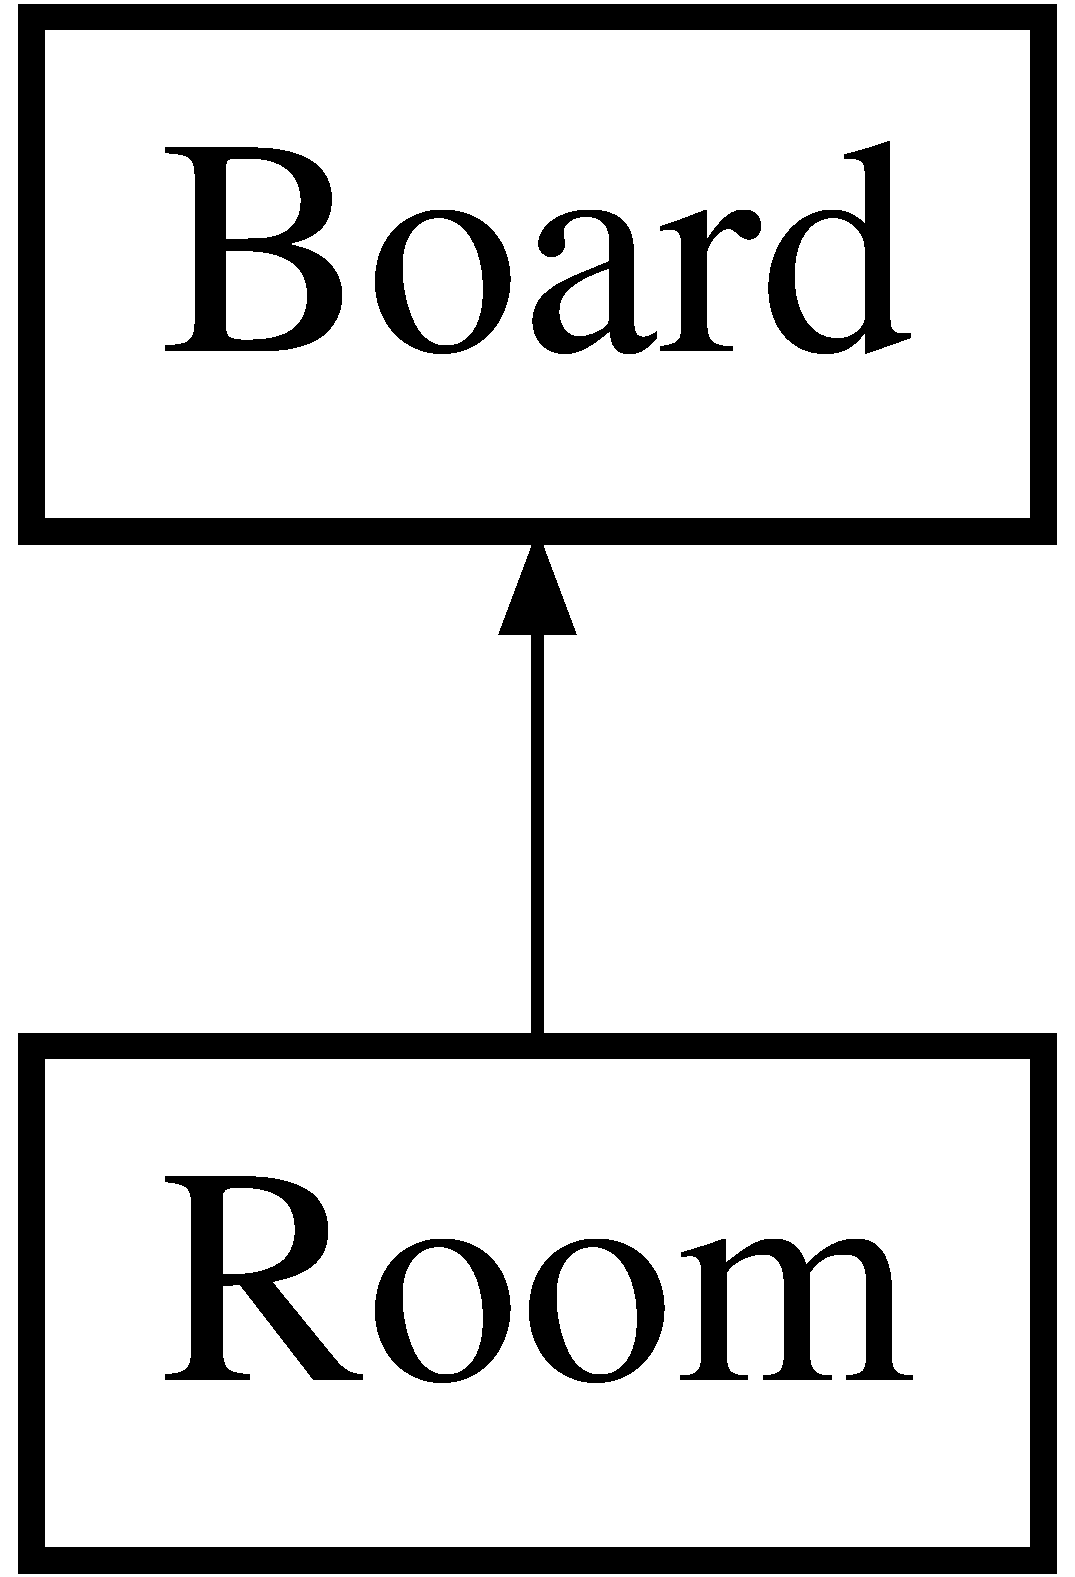
\includegraphics[height=2.000000cm]{classRoom}
\end{center}
\end{figure}
\subsection*{Public Member Functions}
\begin{DoxyCompactItemize}
\item 
int \hyperlink{classRoom_a0874cfd65ae662d303a76cf41d75ff54}{get\-Enemies} ()
\item 
int \hyperlink{classRoom_a4d403f9462e33100386c8f5212c86da5}{get\-Items} ()
\item 
int \hyperlink{classRoom_a0e6d02591ec2e376c91491a12a6bd7d1}{get\-Puzzles} ()
\item 
int \hyperlink{classRoom_a3b09aeaa36969f07f3571168b41b968a}{check\-Location} (int x, int y)
\item 
void \hyperlink{classRoom_a3470492d06e02fc83d696b49f2e9be7d}{set\-Enemies} (int x, int y)
\item 
void \hyperlink{classRoom_aeecd8c82b6670162ae42c619f4dd3f75}{set\-Items} (int x, int y)
\item 
void \hyperlink{classRoom_a185fc0aa127402dc97e092503e10f641}{set\-Puzzles} (int x, int y)
\item 
string \hyperlink{classRoom_a3dc925e6ea4c3e3f671b00307f53ebcd}{Display\-Story} ()
\item 
\hyperlink{classRoom_ac6ef93a7d9c3e1d624e025058d5f16ff}{Room} ()
\item 
\hyperlink{classRoom_a94326fb4bc4d1ad2c88e75d4211f8814}{Room} (int Size\-X, int Size\-Y, string story)
\end{DoxyCompactItemize}
\subsection*{Public Attributes}
\begin{DoxyCompactItemize}
\item 
vector$<$ int $>$ \hyperlink{classRoom_a4b5fb6919c7e49d667f7354008503be5}{Num\-Enemies}
\item 
vector$<$ int $>$ \hyperlink{classRoom_a8b38e13368e3385e52f52160ce896425}{Num\-Items}
\item 
vector$<$ int $>$ \hyperlink{classRoom_a3b1cde750b4a871c6c077c75355d3baa}{Num\-Puzzles}
\item 
string \hyperlink{classRoom_a6b940c409515c78e35eaa50e28a3d2d6}{Story}
\end{DoxyCompactItemize}
\subsection*{Friends}
\begin{DoxyCompactItemize}
\item 
class \hyperlink{classRoom_a6b33a1839e354ea2276f49c4b492ebcb}{Map\-Interface}
\end{DoxyCompactItemize}


\subsection{Constructor \& Destructor Documentation}
\hypertarget{classRoom_ac6ef93a7d9c3e1d624e025058d5f16ff}{\index{Room@{Room}!Room@{Room}}
\index{Room@{Room}!Room@{Room}}
\subsubsection[{Room}]{\setlength{\rightskip}{0pt plus 5cm}Room\-::\-Room (
\begin{DoxyParamCaption}
{}
\end{DoxyParamCaption}
)}}\label{classRoom_ac6ef93a7d9c3e1d624e025058d5f16ff}
\hypertarget{classRoom_a94326fb4bc4d1ad2c88e75d4211f8814}{\index{Room@{Room}!Room@{Room}}
\index{Room@{Room}!Room@{Room}}
\subsubsection[{Room}]{\setlength{\rightskip}{0pt plus 5cm}Room\-::\-Room (
\begin{DoxyParamCaption}
\item[{int}]{Size\-X, }
\item[{int}]{Size\-Y, }
\item[{string}]{story}
\end{DoxyParamCaption}
)}}\label{classRoom_a94326fb4bc4d1ad2c88e75d4211f8814}
\begin{DoxyPrecond}{Precondition}
0=$<$size\-Y\&size\-X$<$=10 
\end{DoxyPrecond}
\begin{DoxyPostcond}{Postcondition}
creates a room 
\end{DoxyPostcond}

\begin{DoxyParams}{Parameters}
{\em sizex} & is x-\/coord, sizey is y-\/coord, string is the story content \\
\hline
\end{DoxyParams}


\subsection{Member Function Documentation}
\hypertarget{classRoom_a3b09aeaa36969f07f3571168b41b968a}{\index{Room@{Room}!check\-Location@{check\-Location}}
\index{check\-Location@{check\-Location}!Room@{Room}}
\subsubsection[{check\-Location}]{\setlength{\rightskip}{0pt plus 5cm}int Room\-::check\-Location (
\begin{DoxyParamCaption}
\item[{int}]{x, }
\item[{int}]{y}
\end{DoxyParamCaption}
)}}\label{classRoom_a3b09aeaa36969f07f3571168b41b968a}
\begin{DoxyPrecond}{Precondition}
location exists 
\end{DoxyPrecond}
\begin{DoxyPostcond}{Postcondition}
returns if you've stepped on an item, enemy, or puzzle 
\end{DoxyPostcond}

\begin{DoxyParams}{Parameters}
{\em int} & x for x-\/coord, int y for y-\/coord \\
\hline
\end{DoxyParams}
\begin{DoxyReturn}{Returns}
int 
\end{DoxyReturn}
\hypertarget{classRoom_a3dc925e6ea4c3e3f671b00307f53ebcd}{\index{Room@{Room}!Display\-Story@{Display\-Story}}
\index{Display\-Story@{Display\-Story}!Room@{Room}}
\subsubsection[{Display\-Story}]{\setlength{\rightskip}{0pt plus 5cm}string Room\-::\-Display\-Story (
\begin{DoxyParamCaption}
{}
\end{DoxyParamCaption}
)}}\label{classRoom_a3dc925e6ea4c3e3f671b00307f53ebcd}
\begin{DoxyPrecond}{Precondition}
none 
\end{DoxyPrecond}
\begin{DoxyPostcond}{Postcondition}
displays story content 
\end{DoxyPostcond}
\hypertarget{classRoom_a0874cfd65ae662d303a76cf41d75ff54}{\index{Room@{Room}!get\-Enemies@{get\-Enemies}}
\index{get\-Enemies@{get\-Enemies}!Room@{Room}}
\subsubsection[{get\-Enemies}]{\setlength{\rightskip}{0pt plus 5cm}int Room\-::get\-Enemies (
\begin{DoxyParamCaption}
{}
\end{DoxyParamCaption}
)}}\label{classRoom_a0874cfd65ae662d303a76cf41d75ff54}
\begin{DoxyPrecond}{Precondition}
enemies exist 
\end{DoxyPrecond}
\begin{DoxyPostcond}{Postcondition}
returns number of enemies in room 
\end{DoxyPostcond}
\begin{DoxyReturn}{Returns}
int 
\end{DoxyReturn}
\hypertarget{classRoom_a4d403f9462e33100386c8f5212c86da5}{\index{Room@{Room}!get\-Items@{get\-Items}}
\index{get\-Items@{get\-Items}!Room@{Room}}
\subsubsection[{get\-Items}]{\setlength{\rightskip}{0pt plus 5cm}int Room\-::get\-Items (
\begin{DoxyParamCaption}
{}
\end{DoxyParamCaption}
)}}\label{classRoom_a4d403f9462e33100386c8f5212c86da5}
\begin{DoxyPrecond}{Precondition}
items exist 
\end{DoxyPrecond}
\begin{DoxyPostcond}{Postcondition}
returns number of items in room 
\end{DoxyPostcond}
\begin{DoxyReturn}{Returns}
int 
\end{DoxyReturn}
\hypertarget{classRoom_a0e6d02591ec2e376c91491a12a6bd7d1}{\index{Room@{Room}!get\-Puzzles@{get\-Puzzles}}
\index{get\-Puzzles@{get\-Puzzles}!Room@{Room}}
\subsubsection[{get\-Puzzles}]{\setlength{\rightskip}{0pt plus 5cm}int Room\-::get\-Puzzles (
\begin{DoxyParamCaption}
{}
\end{DoxyParamCaption}
)}}\label{classRoom_a0e6d02591ec2e376c91491a12a6bd7d1}
\begin{DoxyPrecond}{Precondition}
puzzles exist 
\end{DoxyPrecond}
\begin{DoxyPostcond}{Postcondition}
returns number of puzzles in room 
\end{DoxyPostcond}
\begin{DoxyReturn}{Returns}
int 
\end{DoxyReturn}
\hypertarget{classRoom_a3470492d06e02fc83d696b49f2e9be7d}{\index{Room@{Room}!set\-Enemies@{set\-Enemies}}
\index{set\-Enemies@{set\-Enemies}!Room@{Room}}
\subsubsection[{set\-Enemies}]{\setlength{\rightskip}{0pt plus 5cm}void Room\-::set\-Enemies (
\begin{DoxyParamCaption}
\item[{int}]{x, }
\item[{int}]{y}
\end{DoxyParamCaption}
)}}\label{classRoom_a3470492d06e02fc83d696b49f2e9be7d}
\begin{DoxyPrecond}{Precondition}
location exists, 0=$<$x\&y$<$=10 
\end{DoxyPrecond}
\begin{DoxyPostcond}{Postcondition}
puts an enemy in a location (x,y) 
\end{DoxyPostcond}

\begin{DoxyParams}{Parameters}
{\em int} & x for x-\/coord, int y for y-\/coord \\
\hline
\end{DoxyParams}
\hypertarget{classRoom_aeecd8c82b6670162ae42c619f4dd3f75}{\index{Room@{Room}!set\-Items@{set\-Items}}
\index{set\-Items@{set\-Items}!Room@{Room}}
\subsubsection[{set\-Items}]{\setlength{\rightskip}{0pt plus 5cm}void Room\-::set\-Items (
\begin{DoxyParamCaption}
\item[{int}]{x, }
\item[{int}]{y}
\end{DoxyParamCaption}
)}}\label{classRoom_aeecd8c82b6670162ae42c619f4dd3f75}
\begin{DoxyPrecond}{Precondition}
location exists, 0=$<$x\&y$<$=10 
\end{DoxyPrecond}
\begin{DoxyPostcond}{Postcondition}
puts an item in a location (x,y) 
\end{DoxyPostcond}

\begin{DoxyParams}{Parameters}
{\em int} & x for x-\/coord, int y for y-\/coord \\
\hline
\end{DoxyParams}
\hypertarget{classRoom_a185fc0aa127402dc97e092503e10f641}{\index{Room@{Room}!set\-Puzzles@{set\-Puzzles}}
\index{set\-Puzzles@{set\-Puzzles}!Room@{Room}}
\subsubsection[{set\-Puzzles}]{\setlength{\rightskip}{0pt plus 5cm}void Room\-::set\-Puzzles (
\begin{DoxyParamCaption}
\item[{int}]{x, }
\item[{int}]{y}
\end{DoxyParamCaption}
)}}\label{classRoom_a185fc0aa127402dc97e092503e10f641}
\begin{DoxyPrecond}{Precondition}
location exists, 0=$<$x\&y$<$=10 
\end{DoxyPrecond}
\begin{DoxyPostcond}{Postcondition}
puts a puzzle in a location (x,y) 
\end{DoxyPostcond}

\begin{DoxyParams}{Parameters}
{\em int} & x for x-\/coord, int y for y-\/coord \\
\hline
\end{DoxyParams}


\subsection{Friends And Related Function Documentation}
\hypertarget{classRoom_a6b33a1839e354ea2276f49c4b492ebcb}{\index{Room@{Room}!Map\-Interface@{Map\-Interface}}
\index{Map\-Interface@{Map\-Interface}!Room@{Room}}
\subsubsection[{Map\-Interface}]{\setlength{\rightskip}{0pt plus 5cm}friend class {\bf Map\-Interface}\hspace{0.3cm}{\ttfamily [friend]}}}\label{classRoom_a6b33a1839e354ea2276f49c4b492ebcb}


\subsection{Member Data Documentation}
\hypertarget{classRoom_a4b5fb6919c7e49d667f7354008503be5}{\index{Room@{Room}!Num\-Enemies@{Num\-Enemies}}
\index{Num\-Enemies@{Num\-Enemies}!Room@{Room}}
\subsubsection[{Num\-Enemies}]{\setlength{\rightskip}{0pt plus 5cm}vector$<$int$>$ Room\-::\-Num\-Enemies}}\label{classRoom_a4b5fb6919c7e49d667f7354008503be5}
\hypertarget{classRoom_a8b38e13368e3385e52f52160ce896425}{\index{Room@{Room}!Num\-Items@{Num\-Items}}
\index{Num\-Items@{Num\-Items}!Room@{Room}}
\subsubsection[{Num\-Items}]{\setlength{\rightskip}{0pt plus 5cm}vector$<$int$>$ Room\-::\-Num\-Items}}\label{classRoom_a8b38e13368e3385e52f52160ce896425}
\hypertarget{classRoom_a3b1cde750b4a871c6c077c75355d3baa}{\index{Room@{Room}!Num\-Puzzles@{Num\-Puzzles}}
\index{Num\-Puzzles@{Num\-Puzzles}!Room@{Room}}
\subsubsection[{Num\-Puzzles}]{\setlength{\rightskip}{0pt plus 5cm}vector$<$int$>$ Room\-::\-Num\-Puzzles}}\label{classRoom_a3b1cde750b4a871c6c077c75355d3baa}
\hypertarget{classRoom_a6b940c409515c78e35eaa50e28a3d2d6}{\index{Room@{Room}!Story@{Story}}
\index{Story@{Story}!Room@{Room}}
\subsubsection[{Story}]{\setlength{\rightskip}{0pt plus 5cm}string Room\-::\-Story}}\label{classRoom_a6b940c409515c78e35eaa50e28a3d2d6}


The documentation for this class was generated from the following files\-:\begin{DoxyCompactItemize}
\item 
include/\hyperlink{Room_8h}{Room.\-h}\item 
src/\hyperlink{Room-IMP_8cpp}{Room-\/\-I\-M\-P.\-cpp}\end{DoxyCompactItemize}

\hypertarget{classsave}{\section{save Class Reference}
\label{classsave}\index{save@{save}}
}


{\ttfamily \#include $<$Save\-Function.\-h$>$}

\subsection*{Public Member Functions}
\begin{DoxyCompactItemize}
\item 
void \hyperlink{classsave_a995e1e5f2d96fe1deedb2a1460f1c2df}{S\-A\-V\-E} (\hyperlink{classWonderLand}{Wonder\-Land} \&w)
\item 
void \hyperlink{classsave_aacd3457dd9a8f5326dfb8abf4f2b0902}{L\-O\-A\-D\-X} (\hyperlink{classWonderLand}{Wonder\-Land} \&w)
\end{DoxyCompactItemize}


\subsection{Member Function Documentation}
\hypertarget{classsave_aacd3457dd9a8f5326dfb8abf4f2b0902}{\index{save@{save}!L\-O\-A\-D\-X@{L\-O\-A\-D\-X}}
\index{L\-O\-A\-D\-X@{L\-O\-A\-D\-X}!save@{save}}
\subsubsection[{L\-O\-A\-D\-X}]{\setlength{\rightskip}{0pt plus 5cm}void save\-::\-L\-O\-A\-D\-X (
\begin{DoxyParamCaption}
\item[{{\bf Wonder\-Land} \&}]{w}
\end{DoxyParamCaption}
)}}\label{classsave_aacd3457dd9a8f5326dfb8abf4f2b0902}
\hypertarget{classsave_a995e1e5f2d96fe1deedb2a1460f1c2df}{\index{save@{save}!S\-A\-V\-E@{S\-A\-V\-E}}
\index{S\-A\-V\-E@{S\-A\-V\-E}!save@{save}}
\subsubsection[{S\-A\-V\-E}]{\setlength{\rightskip}{0pt plus 5cm}void save\-::\-S\-A\-V\-E (
\begin{DoxyParamCaption}
\item[{{\bf Wonder\-Land} \&}]{w}
\end{DoxyParamCaption}
)}}\label{classsave_a995e1e5f2d96fe1deedb2a1460f1c2df}


The documentation for this class was generated from the following files\-:\begin{DoxyCompactItemize}
\item 
include/\hyperlink{SaveFunction_8h}{Save\-Function.\-h}\item 
src/\hyperlink{SaveFunction_8cpp}{Save\-Function.\-cpp}\end{DoxyCompactItemize}

\hypertarget{classWonderLand}{\section{Wonder\-Land Class Reference}
\label{classWonderLand}\index{Wonder\-Land@{Wonder\-Land}}
}


{\ttfamily \#include $<$Wonder\-Land.\-h$>$}

\subsection*{Public Member Functions}
\begin{DoxyCompactItemize}
\item 
void \hyperlink{classWonderLand_a35461a84515d98e019190367f2a2dcf3}{setlocation} (int x, int y)
\item 
int \hyperlink{classWonderLand_a1d0bd4419622b9a0d8cf138bda6f1210}{getlocation\-X} ()
\item 
int \hyperlink{classWonderLand_a0db5a7412bb278afb1ff0937ac56e55e}{getlocation\-Y} ()
\item 
int \hyperlink{classWonderLand_a21a5fd12238fc3c9023c2a9ad2751a3e}{get\-Room} ()
\item 
void \hyperlink{classWonderLand_a38efa7b2fc2fd3c1c896fe8b4f00951f}{set\-Room} (int i)
\item 
void \hyperlink{classWonderLand_abeeeb2012482cbe66b2b88c7ba636d6f}{set\-Wonderland} (int si\-Ze, int roomnum)
\item 
\hyperlink{classWonderLand_a12fae5a5bbc81821bec5869f82f2f700}{Wonder\-Land} ()
\end{DoxyCompactItemize}
\subsection*{Friends}
\begin{DoxyCompactItemize}
\item 
class \hyperlink{classWonderLand_a6b33a1839e354ea2276f49c4b492ebcb}{Map\-Interface}
\end{DoxyCompactItemize}


\subsection{Constructor \& Destructor Documentation}
\hypertarget{classWonderLand_a12fae5a5bbc81821bec5869f82f2f700}{\index{Wonder\-Land@{Wonder\-Land}!Wonder\-Land@{Wonder\-Land}}
\index{Wonder\-Land@{Wonder\-Land}!WonderLand@{Wonder\-Land}}
\subsubsection[{Wonder\-Land}]{\setlength{\rightskip}{0pt plus 5cm}Wonder\-Land\-::\-Wonder\-Land (
\begin{DoxyParamCaption}
{}
\end{DoxyParamCaption}
)}}\label{classWonderLand_a12fae5a5bbc81821bec5869f82f2f700}


\subsection{Member Function Documentation}
\hypertarget{classWonderLand_a1d0bd4419622b9a0d8cf138bda6f1210}{\index{Wonder\-Land@{Wonder\-Land}!getlocation\-X@{getlocation\-X}}
\index{getlocation\-X@{getlocation\-X}!WonderLand@{Wonder\-Land}}
\subsubsection[{getlocation\-X}]{\setlength{\rightskip}{0pt plus 5cm}int Wonder\-Land\-::getlocation\-X (
\begin{DoxyParamCaption}
{}
\end{DoxyParamCaption}
)}}\label{classWonderLand_a1d0bd4419622b9a0d8cf138bda6f1210}
\hypertarget{classWonderLand_a0db5a7412bb278afb1ff0937ac56e55e}{\index{Wonder\-Land@{Wonder\-Land}!getlocation\-Y@{getlocation\-Y}}
\index{getlocation\-Y@{getlocation\-Y}!WonderLand@{Wonder\-Land}}
\subsubsection[{getlocation\-Y}]{\setlength{\rightskip}{0pt plus 5cm}int Wonder\-Land\-::getlocation\-Y (
\begin{DoxyParamCaption}
{}
\end{DoxyParamCaption}
)}}\label{classWonderLand_a0db5a7412bb278afb1ff0937ac56e55e}
\hypertarget{classWonderLand_a21a5fd12238fc3c9023c2a9ad2751a3e}{\index{Wonder\-Land@{Wonder\-Land}!get\-Room@{get\-Room}}
\index{get\-Room@{get\-Room}!WonderLand@{Wonder\-Land}}
\subsubsection[{get\-Room}]{\setlength{\rightskip}{0pt plus 5cm}int Wonder\-Land\-::get\-Room (
\begin{DoxyParamCaption}
{}
\end{DoxyParamCaption}
)}}\label{classWonderLand_a21a5fd12238fc3c9023c2a9ad2751a3e}
\hypertarget{classWonderLand_a35461a84515d98e019190367f2a2dcf3}{\index{Wonder\-Land@{Wonder\-Land}!setlocation@{setlocation}}
\index{setlocation@{setlocation}!WonderLand@{Wonder\-Land}}
\subsubsection[{setlocation}]{\setlength{\rightskip}{0pt plus 5cm}void Wonder\-Land\-::setlocation (
\begin{DoxyParamCaption}
\item[{int}]{x, }
\item[{int}]{y}
\end{DoxyParamCaption}
)}}\label{classWonderLand_a35461a84515d98e019190367f2a2dcf3}
\hypertarget{classWonderLand_a38efa7b2fc2fd3c1c896fe8b4f00951f}{\index{Wonder\-Land@{Wonder\-Land}!set\-Room@{set\-Room}}
\index{set\-Room@{set\-Room}!WonderLand@{Wonder\-Land}}
\subsubsection[{set\-Room}]{\setlength{\rightskip}{0pt plus 5cm}void Wonder\-Land\-::set\-Room (
\begin{DoxyParamCaption}
\item[{int}]{i}
\end{DoxyParamCaption}
)}}\label{classWonderLand_a38efa7b2fc2fd3c1c896fe8b4f00951f}
\hypertarget{classWonderLand_abeeeb2012482cbe66b2b88c7ba636d6f}{\index{Wonder\-Land@{Wonder\-Land}!set\-Wonderland@{set\-Wonderland}}
\index{set\-Wonderland@{set\-Wonderland}!WonderLand@{Wonder\-Land}}
\subsubsection[{set\-Wonderland}]{\setlength{\rightskip}{0pt plus 5cm}void Wonder\-Land\-::set\-Wonderland (
\begin{DoxyParamCaption}
\item[{int}]{si\-Ze, }
\item[{int}]{roomnum}
\end{DoxyParamCaption}
)}}\label{classWonderLand_abeeeb2012482cbe66b2b88c7ba636d6f}


\subsection{Friends And Related Function Documentation}
\hypertarget{classWonderLand_a6b33a1839e354ea2276f49c4b492ebcb}{\index{Wonder\-Land@{Wonder\-Land}!Map\-Interface@{Map\-Interface}}
\index{Map\-Interface@{Map\-Interface}!WonderLand@{Wonder\-Land}}
\subsubsection[{Map\-Interface}]{\setlength{\rightskip}{0pt plus 5cm}friend class {\bf Map\-Interface}\hspace{0.3cm}{\ttfamily [friend]}}}\label{classWonderLand_a6b33a1839e354ea2276f49c4b492ebcb}


The documentation for this class was generated from the following files\-:\begin{DoxyCompactItemize}
\item 
include/\hyperlink{WonderLand_8h}{Wonder\-Land.\-h}\item 
src/\hyperlink{WonderLand-IMP_8cpp}{Wonder\-Land-\/\-I\-M\-P.\-cpp}\end{DoxyCompactItemize}

\chapter{File Documentation}
\hypertarget{Board_8h}{\section{include/\-Board.h File Reference}
\label{Board_8h}\index{include/\-Board.\-h@{include/\-Board.\-h}}
}
{\ttfamily \#include $<$array$>$}\\*
{\ttfamily \#include $<$iostream$>$}\\*
{\ttfamily \#include $<$cstdlib$>$}\\*
\subsection*{Classes}
\begin{DoxyCompactItemize}
\item 
class \hyperlink{classBoard}{Board}
\end{DoxyCompactItemize}

\hypertarget{Characters_8h}{\section{include/\-Characters.h File Reference}
\label{Characters_8h}\index{include/\-Characters.\-h@{include/\-Characters.\-h}}
}
{\ttfamily \#include \char`\"{}Map\-Interface.\-h\char`\"{}}\\*
{\ttfamily \#include $<$string$>$}\\*
\subsection*{Classes}
\begin{DoxyCompactItemize}
\item 
class \hyperlink{classMapInterface1}{Map\-Interface1}
\item 
class \hyperlink{classCharacters}{Characters}
\end{DoxyCompactItemize}


\subsection{Detailed Description}
\begin{DoxyAuthor}{Author}
Nicole Vachon 
\end{DoxyAuthor}

\hypertarget{Helpers_8h}{\section{include/\-Helpers.h File Reference}
\label{Helpers_8h}\index{include/\-Helpers.\-h@{include/\-Helpers.\-h}}
}
{\ttfamily \#include $<$string$>$}\\*
\subsection*{Classes}
\begin{DoxyCompactItemize}
\item 
class \hyperlink{classHelpers}{Helpers}
\end{DoxyCompactItemize}

\hypertarget{Items_8h}{\section{include/\-Items.h File Reference}
\label{Items_8h}\index{include/\-Items.\-h@{include/\-Items.\-h}}
}
{\ttfamily \#include \char`\"{}Characters.\-h\char`\"{}}\\*
\subsection*{Classes}
\begin{DoxyCompactItemize}
\item 
class \hyperlink{classItems}{Items}
\end{DoxyCompactItemize}

\hypertarget{MapInterface_8h}{\section{include/\-Map\-Interface.h File Reference}
\label{MapInterface_8h}\index{include/\-Map\-Interface.\-h@{include/\-Map\-Interface.\-h}}
}
{\ttfamily \#include $<$string$>$}\\*
{\ttfamily \#include $<$cstdlib$>$}\\*
\subsection*{Classes}
\begin{DoxyCompactItemize}
\item 
class \hyperlink{classMapInterface}{Map\-Interface}
\end{DoxyCompactItemize}


\subsection{Detailed Description}
\begin{DoxyAuthor}{Author}
Thomas Richardson 
\end{DoxyAuthor}

\hypertarget{puzzles_8h}{\section{include/puzzles.h File Reference}
\label{puzzles_8h}\index{include/puzzles.\-h@{include/puzzles.\-h}}
}
{\ttfamily \#include $<$string$>$}\\*
\subsection*{Classes}
\begin{DoxyCompactItemize}
\item 
class \hyperlink{classPuzzles}{Puzzles}
\end{DoxyCompactItemize}

\hypertarget{Room_8h}{\section{include/\-Room.h File Reference}
\label{Room_8h}\index{include/\-Room.\-h@{include/\-Room.\-h}}
}
{\ttfamily \#include $<$vector$>$}\\*
{\ttfamily \#include $<$string$>$}\\*
{\ttfamily \#include $<$iostream$>$}\\*
{\ttfamily \#include $<$cstdlib$>$}\\*
{\ttfamily \#include \char`\"{}Board.\-h\char`\"{}}\\*
\subsection*{Classes}
\begin{DoxyCompactItemize}
\item 
class \hyperlink{classRoom}{Room}
\end{DoxyCompactItemize}


\subsection{Detailed Description}
\begin{DoxyAuthor}{Author}
Thomas Richardson 
\end{DoxyAuthor}

\hypertarget{SaveFunction_8h}{\section{include/\-Save\-Function.h File Reference}
\label{SaveFunction_8h}\index{include/\-Save\-Function.\-h@{include/\-Save\-Function.\-h}}
}
{\ttfamily \#include \char`\"{}iostream\char`\"{}}\\*
{\ttfamily \#include \char`\"{}Wonder\-Land.\-h\char`\"{}}\\*
{\ttfamily \#include \char`\"{}fstream\char`\"{}}\\*
\subsection*{Classes}
\begin{DoxyCompactItemize}
\item 
class \hyperlink{classsave}{save}
\end{DoxyCompactItemize}

\hypertarget{WonderLand_8h}{\section{include/\-Wonder\-Land.h File Reference}
\label{WonderLand_8h}\index{include/\-Wonder\-Land.\-h@{include/\-Wonder\-Land.\-h}}
}
{\ttfamily \#include \char`\"{}Room.\-h\char`\"{}}\\*
\subsection*{Classes}
\begin{DoxyCompactItemize}
\item 
class \hyperlink{classWonderLand}{Wonder\-Land}
\end{DoxyCompactItemize}

\hypertarget{Characters_8cpp}{\section{src/\-Characters.cpp File Reference}
\label{Characters_8cpp}\index{src/\-Characters.\-cpp@{src/\-Characters.\-cpp}}
}
{\ttfamily \#include \char`\"{}Characters.\-h\char`\"{}}\\*
{\ttfamily \#include $<$iostream$>$}\\*
{\ttfamily \#include $<$cstdlib$>$}\\*
{\ttfamily \#include $<$string$>$}\\*

\hypertarget{Helpers_8cpp}{\section{src/\-Helpers.cpp File Reference}
\label{Helpers_8cpp}\index{src/\-Helpers.\-cpp@{src/\-Helpers.\-cpp}}
}
{\ttfamily \#include \char`\"{}Helpers.\-h\char`\"{}}\\*
{\ttfamily \#include $<$iostream$>$}\\*

\hypertarget{Items_8cpp}{\section{src/\-Items.cpp File Reference}
\label{Items_8cpp}\index{src/\-Items.\-cpp@{src/\-Items.\-cpp}}
}
{\ttfamily \#include \char`\"{}Items.\-h\char`\"{}}\\*
{\ttfamily \#include \char`\"{}Characters.\-h\char`\"{}}\\*
{\ttfamily \#include \char`\"{}iostream\char`\"{}}\\*
{\ttfamily \#include \char`\"{}cstdlib\char`\"{}}\\*

\hypertarget{MapInterface-IMP_8cpp}{\section{src/\-Map\-Interface-\/\-I\-M\-P.cpp File Reference}
\label{MapInterface-IMP_8cpp}\index{src/\-Map\-Interface-\/\-I\-M\-P.\-cpp@{src/\-Map\-Interface-\/\-I\-M\-P.\-cpp}}
}
{\ttfamily \#include \char`\"{}Map\-Interface.\-h\char`\"{}}\\*
{\ttfamily \#include \char`\"{}Save\-Function.\-h\char`\"{}}\\*
{\ttfamily \#include $<$string$>$}\\*
{\ttfamily \#include $<$iostream$>$}\\*
{\ttfamily \#include $<$cstdlib$>$}\\*
{\ttfamily \#include \char`\"{}Wonder\-Land.\-h\char`\"{}}\\*

\hypertarget{puzzles_8cpp}{\section{src/puzzles.cpp File Reference}
\label{puzzles_8cpp}\index{src/puzzles.\-cpp@{src/puzzles.\-cpp}}
}
{\ttfamily \#include \char`\"{}puzzles.\-h\char`\"{}}\\*
{\ttfamily \#include \char`\"{}iostream\char`\"{}}\\*

\hypertarget{Room-IMP_8cpp}{\section{src/\-Room-\/\-I\-M\-P.cpp File Reference}
\label{Room-IMP_8cpp}\index{src/\-Room-\/\-I\-M\-P.\-cpp@{src/\-Room-\/\-I\-M\-P.\-cpp}}
}
{\ttfamily \#include \char`\"{}Room.\-h\char`\"{}}\\*
{\ttfamily \#include $<$cstdlib$>$}\\*
{\ttfamily \#include $<$vector$>$}\\*

\hypertarget{SaveFunction_8cpp}{\section{src/\-Save\-Function.cpp File Reference}
\label{SaveFunction_8cpp}\index{src/\-Save\-Function.\-cpp@{src/\-Save\-Function.\-cpp}}
}
{\ttfamily \#include \char`\"{}Save\-Function.\-h\char`\"{}}\\*
{\ttfamily \#include $<$iostream$>$}\\*
{\ttfamily \#include $<$fstream$>$}\\*
{\ttfamily \#include $<$cstdlib$>$}\\*
{\ttfamily \#include \char`\"{}Wonder\-Land.\-h\char`\"{}}\\*
{\ttfamily \#include \char`\"{}Room.\-h\char`\"{}}\\*
{\ttfamily \#include \char`\"{}Map\-Interface.\-h\char`\"{}}\\*

\hypertarget{WonderLand-IMP_8cpp}{\section{src/\-Wonder\-Land-\/\-I\-M\-P.cpp File Reference}
\label{WonderLand-IMP_8cpp}\index{src/\-Wonder\-Land-\/\-I\-M\-P.\-cpp@{src/\-Wonder\-Land-\/\-I\-M\-P.\-cpp}}
}
{\ttfamily \#include \char`\"{}Wonder\-Land.\-h\char`\"{}}\\*
{\ttfamily \#include \char`\"{}Room.\-h\char`\"{}}\\*
{\ttfamily \#include $<$array$>$}\\*
{\ttfamily \#include $<$iostream$>$}\\*
{\ttfamily \#include $<$cstdlib$>$}\\*

\hypertarget{WonderMain_8cpp}{\section{src/\-Wonder\-Main.cpp File Reference}
\label{WonderMain_8cpp}\index{src/\-Wonder\-Main.\-cpp@{src/\-Wonder\-Main.\-cpp}}
}
{\ttfamily \#include \char`\"{}Helpers.\-h\char`\"{}}\\*
{\ttfamily \#include \char`\"{}Characters.\-h\char`\"{}}\\*
{\ttfamily \#include \char`\"{}Map\-Interface.\-h\char`\"{}}\\*
{\ttfamily \#include \char`\"{}puzzles.\-h\char`\"{}}\\*
{\ttfamily \#include \char`\"{}Items.\-h\char`\"{}}\\*
{\ttfamily \#include \char`\"{}Room.\-h\char`\"{}}\\*
{\ttfamily \#include \char`\"{}Wonder\-Land.\-h\char`\"{}}\\*
{\ttfamily \#include $<$iostream$>$}\\*
\subsection*{Functions}
\begin{DoxyCompactItemize}
\item 
int \hyperlink{WonderMain_8cpp_ae66f6b31b5ad750f1fe042a706a4e3d4}{main} ()
\end{DoxyCompactItemize}
\subsection*{Variables}
\begin{DoxyCompactItemize}
\item 
double \hyperlink{WonderMain_8cpp_a974add80575602303042dfaaa98c7f16}{temp55}
\end{DoxyCompactItemize}


\subsection{Function Documentation}
\hypertarget{WonderMain_8cpp_ae66f6b31b5ad750f1fe042a706a4e3d4}{\index{Wonder\-Main.\-cpp@{Wonder\-Main.\-cpp}!main@{main}}
\index{main@{main}!WonderMain.cpp@{Wonder\-Main.\-cpp}}
\subsubsection[{main}]{\setlength{\rightskip}{0pt plus 5cm}int main (
\begin{DoxyParamCaption}
{}
\end{DoxyParamCaption}
)}}\label{WonderMain_8cpp_ae66f6b31b5ad750f1fe042a706a4e3d4}


\subsection{Variable Documentation}
\hypertarget{WonderMain_8cpp_a974add80575602303042dfaaa98c7f16}{\index{Wonder\-Main.\-cpp@{Wonder\-Main.\-cpp}!temp55@{temp55}}
\index{temp55@{temp55}!WonderMain.cpp@{Wonder\-Main.\-cpp}}
\subsubsection[{temp55}]{\setlength{\rightskip}{0pt plus 5cm}double temp55}}\label{WonderMain_8cpp_a974add80575602303042dfaaa98c7f16}

%--- End generated contents ---

% Index
\newpage
\phantomsection
\addcontentsline{toc}{part}{Index}
\printindex

\end{document}
